\chapter{Design}
The hub can be interacted with in two different ways; on the physical hub or through the website under the energy hub page. In this chapter the different thoughts about the design will be explained.
%%%%%%%%%%%%%%%%%%%%%%%%%%%%%%%%%%%%%%%%%%%%%%
\section{Design Methods - Dennis}
Finding the right design for the hub have been really educational, as two different things to be designed, have given the possibility of trying out different design methods. As the hub is only going to be operated by the customer for the system, it was natural to involve him in the design phase. The participatory design session with the customer is explained in details in the next chapter.
\\As the system is meant as a showoff system, the design of the website is on an experimental level, where pieces from a known operating system have been implemented on a website. The reason not to include users in the design phase of the website has been to come up with a new and innovative design. Whereas most people will stick to something they know if they are supposed to design, for instance a webpage. After the first sketches, both the customer to the system and the web-customer have been contacted to give feedback on the drawings. Later on a usability test was made with the two customers before the creation of the real page. The usability tests is described in details in the next chapter.
\\[0.2cm]
Based on meetings with the two customers, usability goals and user experience goals have been found, to make the final product as close to what they wanted as possible. Experience goals are subjective things which can differ from one person to another based on an opinion or emotion, whereas usability goals are more measurable and not coloured by the persons opinion.
%%%%%%%%%%%%%%%%%%%%%%%%%%%%%%%%%%%%%%%%%%%%%%
\subsection{Usability goals - Dennis}
Based on the meetings points is given to different usability goals due to their priority. 
The below sections will be given points on a scale from 1 to 10 (were 10 is very important and 1 is less important)
\begin{itemize}
	\item 10 safe to use (safety)
	\item 8 easy to learn (learnability) 
	\item 8 easy to remember how to use (memorability)
	\item 6 effective to use (effectiveness) 
	\item 5 efficient to use (efficiency/performance)
	\item 2 have good utility (utility)	
\end{itemize}
\paragraph{Safety}
Most important is the safety factor as the user of the system (Jan) should be able to show the system for high-school students and others, without fiddle-fingers is hurt. Therefore everything dangerous such as: high voltage connections and sharp edges should be held inside the module boxes.
Non-technically experienced persons should also be able to connect devices to the system, without thinking about safety risks. 
\paragraph{Learnability:}
As the system is meant to be operated by a non-technically persons, learning the system shall be fast and operating the system shall therefore be very intuitive. 
Also visitors should be able to do simple tasks on the system, such as turn a device on or off.
\paragraph{Memorability:}
Mainly the system is supposed to run by it self without any interaction. But when the system is going to be operated on, or the system is showed for visitors, the instructed person(s) shall be able to do so without any preparation time.
\paragraph{Effectiveness:}
The effectiveness of the system is not the most important factor, but still quite important as the talk is about a green system, which must be
affordable for the user to implement the system. When investing in a green system, it will have information about estimated lifetime and buy time (the time it takes the system to `buy home itself'). If the buy time is to long, maybe longer than the lifetime, the price for having such a system will be way to high. The goal is that visitors can see the advantage in buying a green system (environmental and money friendly), so it might affect them to be more environmental friendly. 
\paragraph{Efficiency/Performance:}
The performance in the system is not critical when considering it from the users perspective. It doesn't matter if it takes a few seconds before the system responds the user. But for safety reasons it have to operate very fast between the modules so no parts is harmed due to too long response time. But nothing that has directly connection to the user interaction.
\paragraph{Utility:}
The possibility of changing parameters in the system should be kept as low as possible to easy the interaction with the system. If the user have too many ways of setting up the system it can easily confuse more than necessary. Therefore only the most important things that the user should be able to change is implemented, rest of the settings is placed as hidden utilities (only to be set up by the developers during tests). 
%%%%%%%%%%%%%%%%%%%%%%%%%%%%%%%%%%%%%%%%%%%%%%
\subsection{User experience goals - Dennis}
The user should not find this system specially emotional or fun as the system might be seen as frivolous if it is overdone. However, to keep the interest of the visitors (primarily high school students), the system should be entertaining to a certain level.  
Down below the different user experience goals found interesting for the hub are listed in order (most important at the top):
\begin{enumerate}
	\item Rewarding
	\item Helpful
	\item Entertaining
	\item Motivating
	\item Enjoyable
	\item Fun
\end{enumerate}
%\begin{wrapfigure}{r}{0.4\textwidth}
%	\center
%		\setlength\fboxsep{0pt}
%		\setlength\fboxrule{0pt}
%		\fbox{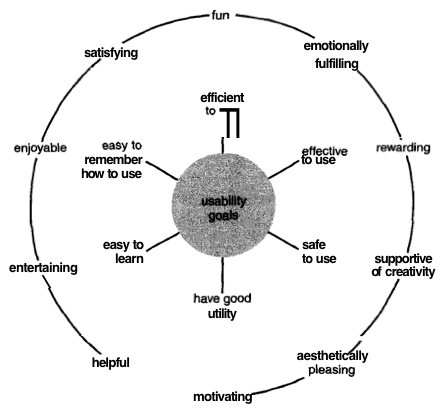
\includegraphics[width=0.4\textwidth]{images/usability_goals_diagram.png}}
%   	\caption{\textit{The difference between usability and user experience goals, where  usability goals are central to
%  			interaction design and are operationalized through specific criteria. 
%  			User experience goals are shown in the outer circle and are less clearly defined.}}
%   	\label{fig:index_page_design}
%\end{wrapfigure}
%\textbf{ }\\ \\
The goal is to give visitors a better understanding of the term 'Green Energy'. They should feel they have become rewarded on the area after having interacted with the system. The system should be helpful, to easy the process of doing things, like seeing the production historic, connected modules etc. The values represented are represented as non-technically expressions to make it more entertaining and to not make the user lose motivation. Even though the user have to learn something by using the system, the system is also supposed be enjoyable and fun to use.
%%%%%%%%%%%%%%%%%%%%%%%%%%%%%%%%%%%%%%%%%%%%%%

\section{Metaphors - Paulo}